\documentclass[a4paper,12pt]{extarticle}
\usepackage{geometry}
\usepackage[T1]{fontenc}
\usepackage[utf8]{inputenc}
\usepackage[english,russian]{babel}
\usepackage{amsmath}
\usepackage{amsthm}
\usepackage{amssymb}
\usepackage{fancyhdr}
\usepackage{setspace}
\usepackage{graphicx}
\usepackage{colortbl}
\usepackage{tikz}
\usepackage{pgf}
\usepackage{subcaption}
\usepackage{listings}
\usepackage{xcolor}
\usepackage{indentfirst}
\usepackage[
backend=biber,
style=numeric,
maxbibnames=99
]{biblatex}
\addbibresource{refs.bib}
\usepackage[colorlinks,citecolor=blue,linkcolor=blue,bookmarks=false,hypertexnames=true, urlcolor=blue]{hyperref} 
\usepackage{indentfirst}
\usepackage{mathtools}
\usepackage{booktabs}
\usepackage[flushleft]{threeparttable}
\usepackage{tablefootnote}

\usepackage{chngcntr} % нумерация графиков и таблиц по секциям
\usepackage{pdfpages}

\counterwithin{table}{section}
\counterwithin{figure}{section}

\graphicspath{{figures/}}

\makeatletter
% \renewcommand{\@biblabel}[1]{#1.} % Заменяем библиографию с квадратных скобок на точку:
\makeatother

\geometry{left=2.5cm}% левое поле
\geometry{right=1.0cm}% правое поле
\geometry{top=2.0cm}% верхнее поле
\geometry{bottom=2.0cm}% нижнее поле
\setlength{\parindent}{1.25cm}
\renewcommand{\baselinestretch}{1.5} % междустрочный интервал


\newcommand{\bibref}[3]{\hyperlink{#1}{#2 (#3)}} % biblabel, authors, year
\addto\captionsrussian{\def\refname{Список литературы (или источников)}} 

\renewcommand{\theenumi}{\arabic{enumi}}% Меняем везде перечисления на цифра.цифра
\renewcommand{\labelenumi}{\arabic{enumi}}% Меняем везде перечисления на цифра.цифра
\renewcommand{\theenumii}{.\arabic{enumii}}% Меняем везде перечисления на цифра.цифра
\renewcommand{\labelenumii}{\arabic{enumi}.\arabic{enumii}.}% Меняем везде перечисления на цифра.цифра
\renewcommand{\theenumiii}{.\arabic{enumiii}}% Меняем везде перечисления на цифра.цифра
\renewcommand{\labelenumiii}{\arabic{enumi}.\arabic{enumii}.\arabic{enumiii}.}% Меняем везде перечисления на цифра.цифра

% Define colors
\definecolor{codegreen}{rgb}{0,0.6,0}
\definecolor{codegray}{rgb}{0.5,0.5,0.5}
\definecolor{codepurple}{rgb}{0.58,0,0.82}
\definecolor{backcolour}{rgb}{0.95,0.95,0.92}

% Setup listings style for Python
\lstdefinestyle{mystyle}{
    language=Python,
    lineskip=-1pt,                   % Немного уменьшаем межстрочный интервал
    frame=single,                    % Рамка вокруг кода
    numbers=left,                    % Нумерация строк слева
    numberstyle=\tiny,               % Стиль номеров строк
    stepnumber=1,                    % Номеровать каждую строку
    numbersep=5pt,                   % Отступ между номерами строк и кодом
    tabsize=4,                       % Размер табуляции
    breaklines=true,                 % Перенос длинных строк
    breakatwhitespace=true,           % Перенос только по пробелам
    showstringspaces=false,           % Не показывать пробелы в строках
    captionpos=b,                    % Подпись снизу
    xleftmargin=1.5em,                % Поля слева
    xrightmargin=1.5em,               % Поля справа
    framexleftmargin=1.5em,           % Чтобы номера строк оказались внутри рамки
    backgroundcolor=\color{backcolour},
    commentstyle=\color{codegreen},
    keywordstyle=\color{magenta},
    numberstyle=\tiny\color{codegray},
    stringstyle=\color{codepurple},
    basicstyle=\ttfamily\footnotesize,
    keepspaces=true,
    showspaces=false,
    showtabs=false,
}
\lstset{style=mystyle} % Apply this style by default


\begin{document}
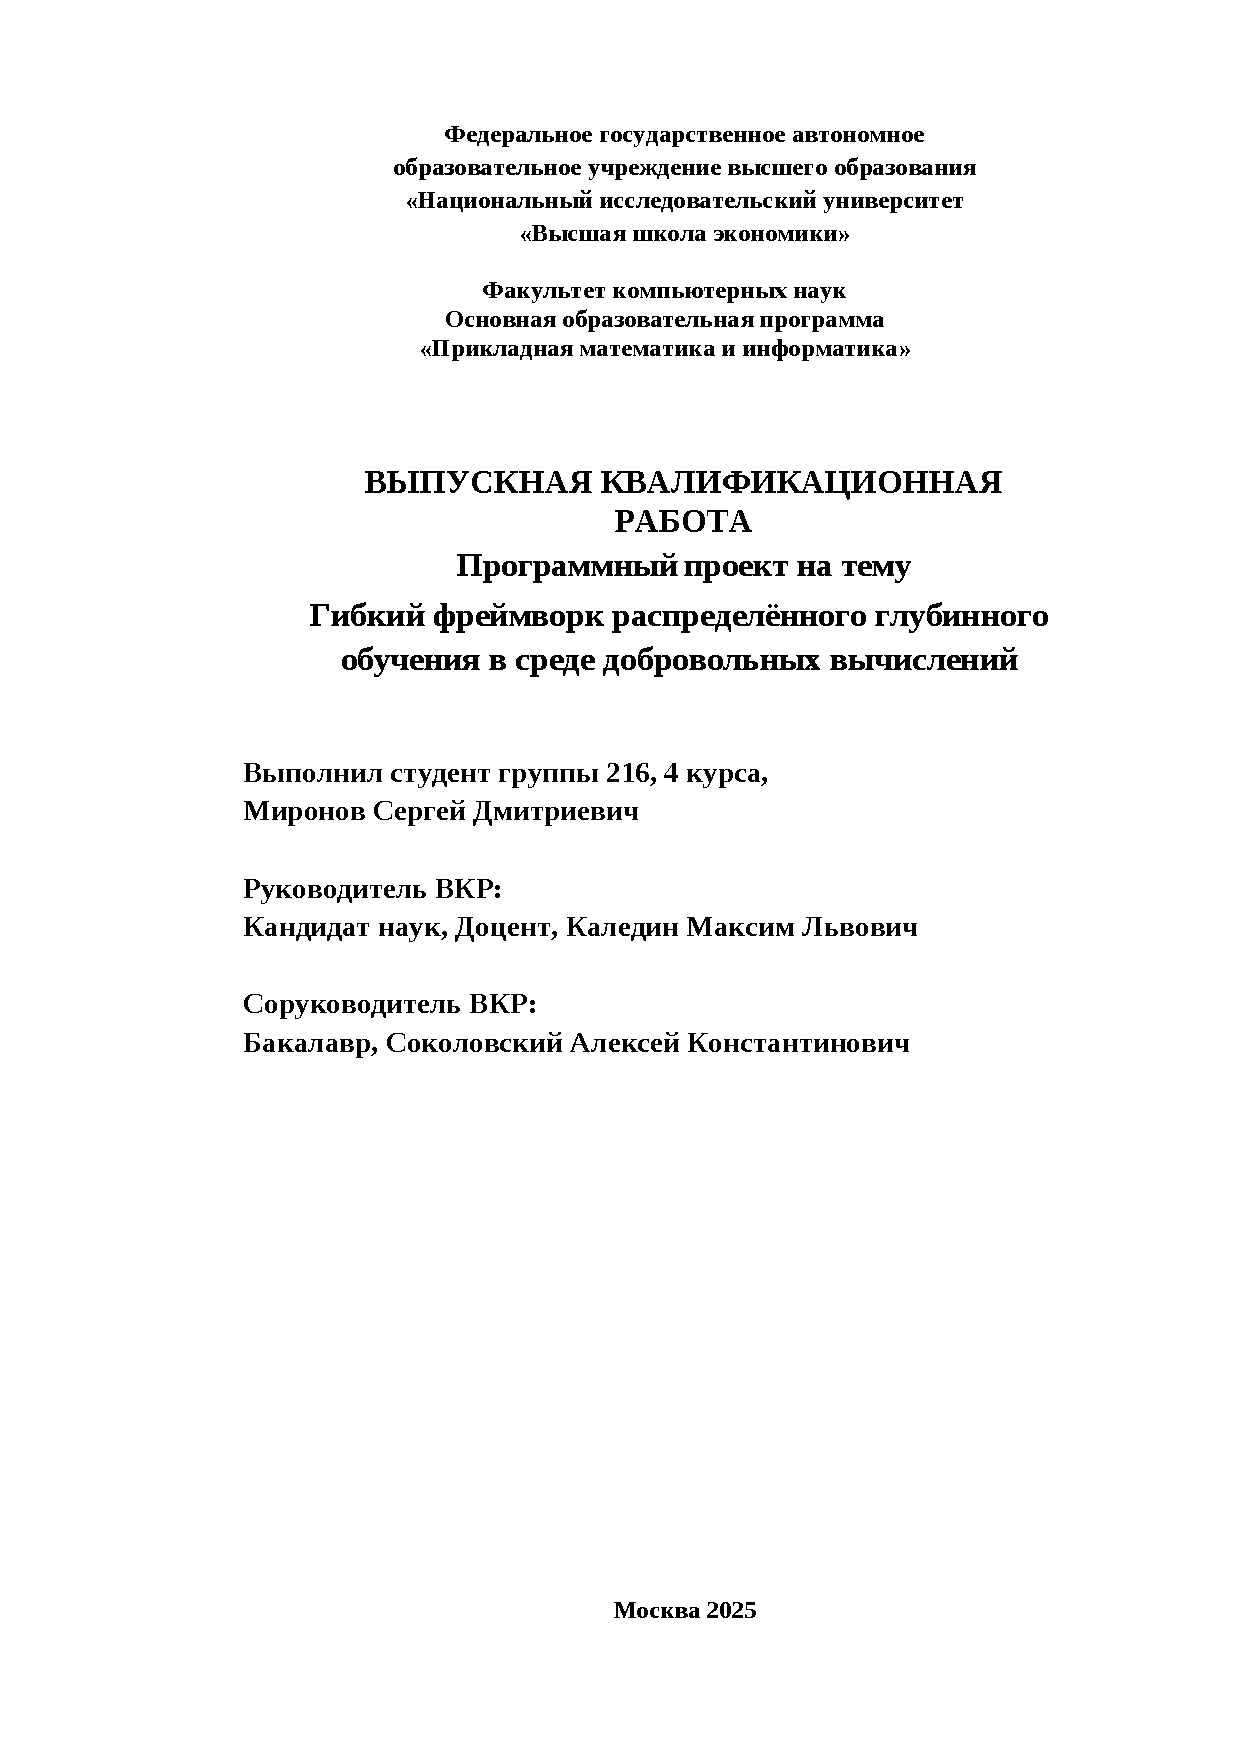
\includepdf[pages=-]{diploma_title_page_1.pdf}
\newpage
\setcounter{page}{2}

{
	\hypersetup{linkcolor=black}
	\tableofcontents
}

\newpage

\section*{Аннотация}

Современные модели глубинного обучения выросли до размеров, при которых их сложно обучить на одном устройстве, а использование кластера может являться дорогостоящим и требовать от исследователей навыков работы с распределёнными системами, что усложняет научную работу в данной области. Для решения этих проблем мы предлагаем STOILO (System for Training Over Independent Learning Operators) — гибкий фреймворк распределённого глубинного обучения на Python, работающий в парадигме добровольных вычислений на базе middleware BOINC. Мы описываем и обосновываем архитектуру системы, предоставляем исходный код и демонстрируем, как система может быть применена для решения задач глубинного обучения. Основным результатом работы является создание удобного и практически применимого фреймворка для выполнения произвольных Python-задач в сети, основанной на платформе BOINC. Предложенное решение может быть адаптировано для широкого круга прикладных проектов.

\section*{Abstract}

Modern deep learning models have grown to a size where they are difficult to train on a single machine, and using a cluster can be expensive and require researchers to be skilled in distributed systems, making research in this area difficult. To address these challenges, we propose STOILO (System for Training Over Independent Learning Operators) — a flexible distributed deep learning framework in Python that operates in a volunteer computing paradigm based on the BOINC middleware. We describe and justify the architecture of the system, provide the system source code, and demonstrate how the system can be applied to deep learning tasks. The main outcome of this work is the creation of a convenient and practically applicable framework for executing arbitrary Python tasks within a net based on the BOINC. The proposed solution can be adapted for a wide range of applied projects.

\addcontentsline{toc}{section}{Аннотация}
\addcontentsline{toc}{section}{Abstract}

\section*{Ключевые слова}
Распределённое глубинное обучение, BOINC, Python Master-Worker

\pagebreak

% введение, обзор литературы, постановка задачи и описание вашего подхода
\section{Введение}

Машинное обучение, а особенно его направление — глубинное обучение, — является быстроразвивающейся и крайне перспективной областью компьютерных наук.
Глубинное обучение помогает решать широкий спектр сложных задач: от распознавания объектов на изображениях и видео до генерации естественного текста и диагностики заболеваний по медицинским снимкам.
Однако выдающиеся модели глубинного обучения часто обладают большими размерами: они содержат миллионы параметров и требуют выполнения значительного количества вычислительных операций.
Например, ResNet-152 — современная нейросетевая архитектура для классификации изображений — имеет более 60 миллионов параметров и предполагает выполнение сотен миллиардов операций с числами с плавающей точкой (FLOPS) в процессе обучения~\cite{he2015deepresidual}.
Кроме того, такие модели требуют объёмных датасетов для обучения. Таким образом, модели, демонстрирующие высококачественные результаты, предъявляют серьёзные требования к вычислительным ресурсам. Ресурсов одной машины быстро становится недостаточно, а построение классических решений в виде on-premises или облачных кластеров является финансово затратным.

В рамках данного проекта мы предлагаем STOILO (System for Training Over Indepen-\\dent Learning Operators) — систему распределённого машинного обучения, основанную на концепции добровольных вычислений — модели, в которой пользователи предоставляют недоиспользованные ресурсы своих устройств научным исследованиям из альтруистических соображений.
Важным требованием к создаваемой системе является простота и гибкость в использовании: с её помощью должно быть возможно и удобно обучать произвольные модели глубинного обучения.

Исходный код системы опубликован в github репозитории автора и доступен по ссылке \url{https://github.com/sermir2003/stoilo}.

\section{Системы добровольных и grid вычислений}

Добровольные вычисления (англ. \textit{Volunteer Computing, VC}) — это модель распределённых вычислений, в которой владельцы персональных устройств предоставляют их недоиспользованные ресурсы научным проектам на безвозмездной основе.
Устройства добровольцев обрабатывают отдельные задачи крупных исследований в фоновом режиме, формируя мощную распределённую систему.
Такой подход позволяет существенно сократить расходы на вычислительные мощности и задействовать ресурсы, на которые не обращают внимания другие вычислительные парадигмы~\cite{anderson2020boinc}.

Яркими примерами успешного применения добровольных вычислений являются проекты
\textit{SETI@home}, занимающийся анализом радиосигналов из космоса~\cite{Anderson2002},
\textit{Rosetta@home}, предсказывающий трёхмерные структуры, моделирующий взаимодействия и проектирующий по заданным свойствам белки; результаты, полученные в рамках данного проекта, были использованы при разработке некоторых лекарств и вакцин \cite{RosettaHomeWiki},
\textit{Folding@home}, специализирующийся на моделировании процессов сворачивания белков и внёсший значительный вклад в исследование COVID-19~\cite{Zimmerman2021}.
Перечисленные проекты привлекли сотни тысяч участников по всему миру и наглядно продемонстрировали практическую применимость добровольных вычислений в решении научных задач.

Модель добровольных вычислений тесно связана с концепцией grid-вычислений, направленной на объединение ресурсов нескольких организаций, например институтов, с целью совместного решения сложных задач~\cite{Foster2001}.
Основное отличие добровольных вычислений заключается в отсутствии административного контроля над вычислительными узлами, что порождает дополнительные вопросы безопасности и защиты от злонамеренного поведения.
Кроме того, системы добровольных вычислений изначально рассчитаны на более высокую гетерогенность и широкую географическую распределённость узлов по сравнению с grid-системами.
В некотором смысле добровольные вычисления представляют собой более общий класс распределённых систем, не делающий ряда предположений о свойствах вычислительной среды.
Создание системы на основе добровольных вычислений выглядит крайне привлекательным: подобная архитектура универсальна и при необходимости может быть адаптирована как для использования ресурсов организаций — например, неактивно используемых компьютеров учебных классов университета, — так и для экономичной работы в облачных средах с использованием preemptible instances, стоимость которых на 70–90\% ниже instances со стандартными гарантиями надёжности.

Существует несколько платформ для организации добровольных вычислений:
\begin{itemize}
    \item \textit{BOINC} (Berkeley Open Infrastructure for Network Computing) — универсальная и масштабируемая система, лежащая в основе множества успешных научных проектов~\cite{anderson2020boinc}. 
    \item \textit{Charity Engine} — коммерческая инициатива, использующая модифицированную версию BOINC для монетизации вычислительных мощностей и передачи вырученных средств на благотворительные нужды. 
    \item \textit{DreamLab} — мобильная платформа Vodafone Foundation, позволяющая задействовать вычислительные ресурсы смартфонов для медицинских исследований~\cite{Tapparello2015}.
\end{itemize}

Среди этих платформ \textit{BOINC} является наиболее технически зрелой и распространённой. Её ключевые преимущества включают:

\begin{itemize}
    \item \textit{Поддержку гетерогенных устройств и ускорителей} — выполнение задач на CPU, GPU (через OpenCL и CUDA), а также на мобильных устройствах.
    \item \textit{Развитую инфраструктуру} — планирование заданий в гетерогенной среде, сбор и верификацию результатов, автоматическое управление ресурсами.
    \item \textit{Высокую масштабируемость} — возможна успешная работа с сотнями тысяч узлов и миллионами заданий в день, существует база для горизонтального масштабирования.
    \item \textit{Активную разработку и сообщество} — регулярные обновления, открытый исходный код и множество доступной справочной информации.
\end{itemize}

Фактически BOINC стала стандартом добровольных вычислений: подавляющее большинство современных проектов в этой области основаны именно на данной платформе \cite{Mengistu2019}. Это делает выбор BOINC рациональным для создания новых систем добровольных вычислений, обеспечивая техническую зрелость, гибкость и широкую поддержку.

\section{Системы машинного обучения на основе BOINC}

Существует немало проектов на базе BOINC, связанных с машинным обучением. Ниже рассмотрены несколько наиболее интересных из них, с акцентом на универсальность и удобство их использования для инженеров машинного обучения.

\textbf{MLC@Home} — один из наиболее известных проектов машинного обучения, запущенный в 2020 году Университетом Мэриленда. Его целью было не обучение нейросетей для непосредственного применения, а исследование свойств весов обученных моделей. Добровольцы обучили множество небольших моделей, в результате чего был собран датасет MLDS \cite{Clemens2021}. Хотя проект дал ценные научные данные в области интерпретируемости моделей, он не предоставлял пользователю интерфейс для обучения произвольных нейросетей: архитектура модели была жёстко зафиксирована в C++ коде, и для её изменения требовалось изменение кода проекта.

\textbf{Large Scale Evolution of Convolutional Neural Networks Using VC} — статья 2017 года, в которой был использован алгоритм EXACT для эволюционного построения свёрточных нейросетей~\cite{Desell2017}. Добровольцы обучили различные варианты архитектур, постепенно улучшая их. BOINC позволил провести масштабный перебор моделей, однако, как и в случае с MLC@Home, система была жёстко ориентирована на одну задачу и не предусматривала обучение произвольных моделей, заданных пользователем.

\textbf{DistributedDataMining (dDM)} — проект 2013 года, предлагающий выполнение RapidMiner поверх BOINC \cite{Schlitter2013}. RapidMiner является графической средой для построения пайплайнов анализа данных. В dDM добровольцы через BOINC исполняли сценарии \newline RapidMiner, а результаты собирались на сервере. Такой подход позволил распределённо решать ресурсоёмкие задачи прогнозирования рыночной стоимости акций, анализа медицинских данных и оптимизации моделей машинного обучения. Однако использование системы сопровождалось рядом трудностей: пользователь должен был вручную создать и экспортировать RapidMiner process в формате XML, разумно разбить вычисление на независимые задачи (jobs), подготовить отдельные input/output файлы для каждой задачи и запустить вычисления через BOINC wrapper-программу для RapidMiner. Фактически интегрированного с runtime BOINC интерфейса создано не было, вместо этого предлагалось вручную портировать процессы из RapidMiner на BOINC.

\textbf{Distributed Deep Learning Using Volunteer Computing-Like Paradigm} — статья 2019 года, в которой предложена архитектура распределённого глубинного обучения на базе BOINC~\cite{atre2021distributed}. Авторы реализовали обучение в парадигме Data Parallelism с Parameter Server и предложили схему асинхронного обновления градиентов VC-ASGD. Они обучили несколько нейросетей, продемонстрировав потенциал распределённого обучения в добровольной среде. Однако исходный код системы опубликован не был. Авторы заявили о создании гибкого интерфейса, в котором достаточно средствами TensorFlow определить модель, задать функцию потерь и указать датасет, после чего обучение произойдёт автоматически. Тем не менее полноценного инструмента, готового для конечного применения, предъявлено не было.

Анализ существующих проектов показывает, что платформа BOINC обладает высоким потенциалом для решения задач машинного обучения, позволяя масштабировать ресурсоёмкие вычисления за счёт распределения нагрузки между добровольными участниками. Однако все рассмотренные системы либо ориентированы на выполнение узкой фиксированной задачи, либо требуют значительных технических усилий от пользователя, включая написание кода на C++ и ручную адаптацию процессов под модель BOINC. Существенным достижением в области универсализации является работа Atre и др.~\cite{atre2021distributed}, предложившая архитектуру обучения моделей на основе TensorFlow, однако полноценного инструмента для практического применения опубликовано не было.

\section{Модель вычислений и хранения данных BOINC}

BOINC является middleware с открытым исходным кодом для разработки проектов добровольных вычислений~\cite{anderson2004boinc,anderson2020boinc}. Система на основе BOINC состоит из совокупности серверных процессов (демонов), базы данных MySQL или MariaDB и клиентского программного обеспечения для выполнения заданий на устройствах добровольцев.

Поскольку обычно устройства волонтёров не имеют публичных IP адресов и находятся за NAT, модель BOINC предполагает, что все коммуникации происходят по инициативе клиентов: клиент устанавливает соединение с сервером, информирует о своих ресурсах, запрашивает новые задания и, возможно, доставляет результаты выполненных заданий.

Серверные демоны — это процессы, выполняющие конкретные логические функции и взаимодействующие с базой данных и файловой системой сервера. К ним относятся:
\begin{itemize}
    \item \texttt{work\_generator} — генерирует новые задания, формирует входные данные, оценивает вычислительную сложность и задаёт требования к клиентам;
    \item \texttt{scheduler} — отвечает на сетевые запросы клиентов, принимает результаты и исходя из доступных ресурсов клиента, истории взаимодействия с ним, а также с учётом списка имеющихся задач, их требований к клиентам, предполагаемой сложности и заданных параметров, принимает решение о назначении новых задач;
    \item \texttt{transitioner} — отслеживает состояние заданий и выполняет необходимые действия согласно конечному автомату проекта, например, инициирует новые вычисления, если для некоторого задания собрано недостаточно корректных результатов;
    \item \texttt{validator} — проверяет корректность результатов, выявляет ошибки и зловредное поведение; для защиты от злонамеренного поведения BOINC применяет репликацию вычислений с последующим сравнением полученных результатов, выполняемым validator-ом;
    \item \texttt{assimilator} — обрабатывает валидированные результаты, может, например, сохранять их в базу данных или инициировать последующую обработку;
\end{itemize}
и некоторые другие служебные, например, \texttt{feeder}, \texttt{file\_deleter}, \texttt{db\_purge}.

Важно, что разработчикам проекта на базе BOINC обычно достаточно реализовать только три компонента: \texttt{work\_generator}, \texttt{validator} и \texttt{assimilator} с бизнес-логикой проекта. Остальные демоны предоставляются BOINC.

Помимо серверной части, требуется реализация кода, который будет запускаться клиентом BOINC на узлах добровольцев. В терминологии BOINC различают два понятия: \textit{app} и \textit{app versions}. \textit{app} — это логически индивидуальное приложение, а \textit{app versions} — конкретная семантическая версия приложения для конкретной архитектуры. В качестве иллюстрации приведём пример: приложение может называться \texttt{worker} или \texttt{calculator}, а версия приложения — \texttt{1.0/windows\_x86\_64/worker} или \texttt{3.14/arm-android-linux-gnu/calculator}. Разработчик проекта обязан самостоятельно подготовить версии приложений для всех целевых платформ. В старых выпусках BOINC версия приложения должна была представлять из себя один исполняемый файл, однако в настоящее время BOINC поддерживает комплектацию версий приложений из нескольких файлов, что позволяет запускать приложения через обёртки (wrappers) или внутри виртуальной машины или Docker контейнера.

Что касается управления данными, классическая модель BOINC предполагает взаимодействие клиентов исключительно с центральным сервером. Горизонтальное распределение данных возможно: файлы могут храниться на дополнительных серверах или в отдельных базах данных для повышения масштабируемости, однако BOINC изначально не предусматривает надёжное хранение данных на клиентах или общение клиентов между собой.

Фундаментальным понятием системы является файл: каждый файл в BOINC неизменяем и идентифицируется уникальным именем. В задании указывается список необходимых файлов, а сервер и клиент автоматически управляют их доставкой, хранением и удалением. Влиять на эти процессы можно, например, такими настройками, как \textit{Sticky flag} — не удалять файл после выполнения задания или \textit{Locality scheduling} — учитывать уже загруженные файлы при планировании новых заданий, что позволяет назначать задачи на узлы, где уже присутствует некоторый необходимый объёмный файл.

Проблема масштабируемости передачи данных была рассмотрена в работе Costa и др.~\cite{costa2008optimizing}, где предлагалось использовать протокол BitTorrent для распределённой доставки больших файлов между клиентами. Решение позволило существенно снизить нагрузку на сервер, однако потребовало модификации клиентского программного обеспечения и оказалось не слишком эффективным при малом числе участников в сети и при малых размерах файлов.

Альтернативную архитектуру предложили Foster и др.~\cite{alonso2017new}, внедрив систему хранения данных на подмножестве добровольных узлов (Storage Agents). Такой подход улучшал масштабируемость для задач с большими объёмами данных и высокой географической распределённости, но требовал дополнительной координации (NAT traversal) и надёжного контроля целостности информации, что в значительной мере усложняло архитектуру проекта.

\section{Типы распределённых систем машинного обучения}

Распределённое машинное обучение может проводиться с использованием различных стратегий. Руководствуюсь обзорной статьёй Verbraeken и др.\cite{verbraeken2020survey} и метаанализом Ben-Nun и др.\cite{ben-nun2019demystifying}, основанным на анализе 252 систем и публикаций, описывающих различные аспекты распределённого и параллельного машинного обучения, можно выделить следующие степени свободы архитектур систем машинного обучения.

\begin{description}
    \item[Single-machine Parallelism] — ускорение вычислений за счёт оптимального использования параллелизма и ускорителей на уровне одного узла: многопоточность и многопроцессорность CPU, TPU и GPU.
    
    Разработка собственных низкоуровневых или математических оптимизаций выполнения арифметических операций, возникающих в процессе машинного обучения, не является задачей данной работы. А без глубоких оптимизаций арифметических действий реализовать собственную среду исполнения, сопоставимую по производительности со средами исполнения PyTorch или TensorFlow, не представляется возможным. Поэтому для выполнения операций на уровне одного узла мы используем существующие программные решения.

    \item[Multi-machine Parallelism] — способы распределения работы между несколькими машинами. Возможны следующие подходы:
    \begin{description}
        \item[Data Parallelism] — обучение одной и той же модели на разных подмножествах данных, распределённых между узлами. Этот метод позволяет обрабатывать объёмные датасеты, которые не помещаются на одной машине, при условии, что модель может быть реплицирована на каждый узел.
        \item[Model Parallelism] — разделение вычислительного графа модели между несколькими машинами. Такой подход упрощает обучение больших моделей, однако передача данных прямого и обратного распространений в распределённой среде может представлять существенные накладные расходы.
        \item[Pipelining] — стратегия конвейерной обработки: каждый узел выполняет свою часть последовательности операций над входными данными. Благодаря параллельному выполнению нескольких операций обучения, конвейеризация позволяет повысить загрузку оборудования, использование вычислительных мощностей, но усложняет управление зависимостями и требует надёжной синхронизации.
        \item[Hybrid Parallelism] — произвольная комбинация перечисленных выше методов. Эти подходы не являются взаимоисключающими и могут применяться совместно в зависимости от задачи и инфраструктуры.
    \end{description}

    В рамках данной работы мы ограничиваемся методом Data Parallelism. В отличии от других подходов, под Data Parallelism относительно легко адаптировать существующие фреймворки машинного обучения, включая PyTorch. Кроме того, Data Parallelism не требует передачи большого объёма данных или частой синхронизации между узлами, что делает его более приспособленным для систем, высоко распределённых в географическом отношении, в том числе систем добровольных вычислений.

    \item[Synchronization] — стратегии синхронизации градиентов и весов в процессе выполнения градиентного спуска. Возможные варианты:
    \begin{description}
        \item[Synchronous] — каждый шаг градиентного спуска выполняется строго после сбора и усреднения градиентов от всех вычислительных узлов.
        \item[Stale-Synchronous] — допускается использование устаревших градиентов в пределах фиксированного ``запаздывания''. Это снижает требования к синхронизации при сохранении теоретических гарантий сходимости алгоритма оптимизации.
        \item[Asynchronous] — каждый шаг спуска выполняется на основе градиентов, доступных на данный момент времени. Такой подход уменьшает накладные расходы на синхронизацию, но может негативно сказаться на скорости и качестве сходимости. Вообще говоря, гарантий сходимости у подобного градиентного спуска обычно нет.
        \item[Nondeterministic Communication] — модель, при которой передача градиентов и параметров модели происходит между узлами случайным образом в сложной топологии без строгой синхронизации.
    \end{description}

    Наиболее перспективным выглядит Stale-Synchronous подход. В отличие от полностью синхронного режима, выбранный метод не требует завершения всех заданий текущей эпохи для начала следующей, тем самым избегая колоссального недоиспользования вычислительных мощностей. Более асинхронные методы, хотя и позволяют уменьшить накладные расходы на синхронизацию, заметно жертвуют сходимостью и не гарантируют преимущества в условиях добровольных вычислений.

    \item[Centralization] — способы организации хранения и обновления параметров модели. Возможны следующие архитектуры:
    \begin{description}
        \item[Parameter Server (PS)] — один или несколько выделенных серверов, которые хранят все параметры модели, принимают градиенты от рабочих узлов и отправляют обновлённые веса обратно. Такая архитектура упрощает координацию, но может стать узким местом при высокой нагрузке.
        \item[Sharded PS] — распределение пространства параметров между несколькими серверами. Каждый сервер отвечает только за часть параметров (шард), что позволяет уменьшить нагрузку на сеть и повысить масштабируемость.
        \item[Hierarchical PS] — многоуровневая организация серверов параметров: рабочие узлы взаимодействуют с локальными серверами, которые в свою очередь координируются с центральными серверами. Такая схема снижает сетевые затраты и улучшает масштабируемость в больших кластерах.
        \item[Decentralized] — рабочие узлы напрямую обмениваются градиентами и параметрами друг с другом, без выделенного сервера. Обновления могут происходит посредствам коллективных операций, например, AllReduce, что устраняет единую точку отказа, но требует эффективной синхронизации.
    \end{description}

    В BOINC, как и во многих других системах добровольных вычислений, прибегают к централизованной схеме (PS/Sharded PS), позволяющей определять недобросовестных исполнителей и не требующей коммуникаций между устройствами добровольцев, поведение которых может быть непредсказуемым.
\end{description}

Таким образом, для построения системы в среде добровольных вычислений нам больше всего подходит схема с параллелизмом по обучающим данным (Data Parallelism), синхронизацией параметров модели с ограниченным запаздыванием (Stale-Synchronous) и централизованным сервером параметров (Parameter Server).

\section{Постановка задачи}

Как показал обзор существующих решений, в настоящее время отсутствует универсальная и готовая к практическому применению система распределённого машинного обучения на базе платформы BOINC. Имеющиеся проекты либо ориентированы на решение узкоспециализированных задач, либо требуют от пользователей значительных усилий по интеграции моделей, включая необходимость ручной адаптации к инфраструктуре и написания низкоуровневого кода. В результате существующие системы оказываются малопригодными для широкого круга инженеров машинного обучения, ожидающих простой и привычный интерфейс для построения и обучения моделей.

Целью настоящей работы является разработка системы распределённого машинного обучения на базе BOINC, которая сочетала бы вычислительные возможности добровольной среды с удобством современных фреймворков машинного обучения. Основные требования к системе включают универсальность в отношении типов моделей и задач, удобство для пользователей без необходимости вмешательства в низкоуровневые компоненты, а также возможность эффективного масштабирования в распределённой среде добровольных вычислений.

\section{Описание архитектуры системы}

В данном разделе содержится описание архитектуры созданной нами системы распределённого глубинного обучения STOILO. Система состоит из трёх основных компонентов: пользовательской Python-библиотеки \texttt{stoilo}, сервера проекта на базе BOINC — \texttt{Hlev} и версий приложений для клиентов BOINC \texttt{raboshka\_*}. В последующих подразделах подробно рассматриваются их устройство, функции и обоснование проектных решений.

\begin{figure}[ht]
	\centering
	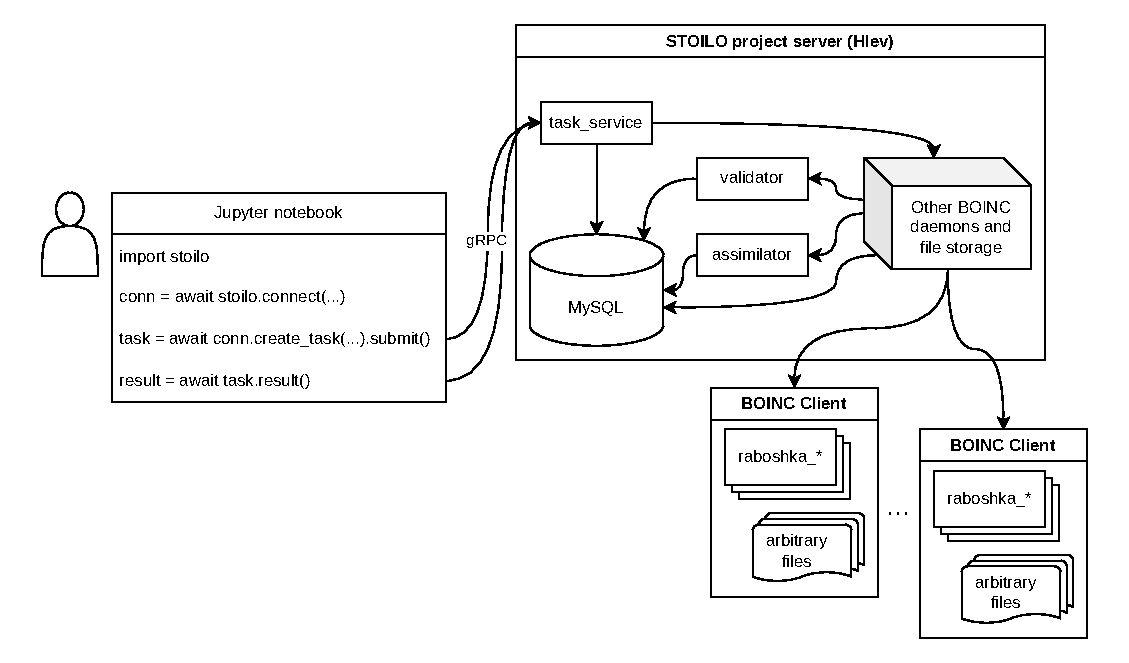
\includegraphics[width=0.8\textwidth]{stoilo_overall.drawio.pdf}
	\caption{Структурная схема STOILO.}
	\label{fig:stoilo_overall}
\end{figure}

\subsection{Пользовательская Python-библиотека}

Пользовательская библиотека \texttt{stoilo} предназначена для взаимодействия с серверной частью системы. Она устанавливает gRPC соединение с сервером и обменивается сообщениями, из которых основные два — это \textit{CreateTask} и \textit{PollTask}. Функции каждого из этих запросов будут подробно рассмотрены ниже.

\subsubsection{Высокоуровневые обёртки для машинного обучения}

Высокоуровневый интерфейс позволяет обучать PyTorch модели через распараллеливание отдельных эпох градиентного спуска.
Фактически это парадигма synchronous data parallelism с parameter server. Идея заключается в том, чтобы разбивать обучение внутри эпохи на независимые задачи, выполняемые на добровольных узлах.

Для наглядности в листинге~\ref{list:example_classic_pytorch} представлен классический mini-batch способ обучения модели с использованием фреймворка PyTorch.

\begin{lstlisting}[caption={Пример классического mini-batch обучения модели с помощью PyTorch.}, label={list:example_classic_pytorch}]
loss_history = []
for epoch in range(num_epochs):
    current_loss = 0
    for inputs, labels in loader:
        optimizer.zero_grad()
        outputs = model(inputs)
        loss = loss_func(outputs, labels)
        loss.backward()
        optimizer.step()
        current_loss += loss.item()
    avg_loss = current_loss / len(loader)
    loss_history.append(avg_loss)
\end{lstlisting}

Предлагаемый интерфейс позволяет заменить вложенный цикл обучения по батчам на вызов функции, автоматически распределяющей обучение модели на каждом батче на узлы распределённой системы, как показано в листинге~\ref{list:example_distributed_training}.

\begin{lstlisting}[caption={Распределённое обучение модели с использованием STOILO}, label={list:example_distributed_training}]
import stoilo

conn = await stoilo.connect(server_address)

trainer = await stoilo.ml.DPBGDTrainer(conn, model, loss_func,
    optimizer_class, optimizer_kwargs, dataset)
loss_history = []
for epoch in range(num_epochs):
    model, avg_loss = await trainer.train_epoch()
    loss_history.append(avg_loss)
\end{lstlisting}

Такой подход не является идиоматичным по отношению к PyTorch, поскольку теряется прямой контроль над конкретными операциями шага обучения, однако, некоторый достаточно высокий уровень гибкости сохраняется: пользователь может задать произвольные модель, функцию потерь, оптимизатор и датасет, а система возьмёт на себя распараллеливание вычислений в пределах каждой эпохи.

В предложенной обёртке обучение реализуется следующим образом: \texttt{.train\_epoch()} случайным образом разделяет датасет на мини-батчи и создаёт для каждого из них задачу, состоящую в вычислению градиентов модели на данном батче. Возвращаемым значением задач являются частичные градиенты, которые затем суммируются и усредняются по количеству мини-батчей. Благодаря этому процессу мы получаем полный градиент модели по всему датасету, после чего совершаем шаг оптимизации с помощью переданного \texttt{optimizer}.

% Датасет передаётся на узлы добровольцев в виде файловой зависимости; предполагается, что каждый BOINC клиент загрузит его один раз, после чего будет использовать локальное хранение, собирая необходимые батчи по индексам из \texttt{call\_spec} файла конкретной задачи. Описанный подход позволяет существенно сократить объём пересылаемых данных между сервером и клиентами и обеспечивает загрузку добровольных ресурсов при сохранении корректности алгоритма обучения.

\subsubsection{Низкоуровневый Python-интерфейс}

Для упрощения работы и снижения порога входа высокоуровневый интерфейс скрывает многие детали реализации и жертвует гибкостью системы.
Не все задачи могут быть решены с его помощью, поэтому более продвинутым пользователям мы предлагаем ``низкоуровневый интерфейс'' \texttt{stoilo}, который позволяет запускать на узлах добровольцев задачи, заключающиеся в выполнении произвольной Python функции. Возвращаемое значение таких Python функций будет доставляться пользователю в качестве результата выполнения задачи. На этом уровне пользователи самостоятельно управляют созданием и отправкой Python-задач на сервер.

В листинге~\ref{list:low_level} приведён пример использования низкоуровневого интерфейса. Для начала устанавливается соединение с сервером, после чего через объект соединения создаются задачи.
Для создания новой задачи используется метод \texttt{Connection.create\_task(\ldots)}, основными аргументами которого являются \texttt{func} — Python-объект типа \texttt{Callable[[Dict[str, Any]], Any]}, представляющий собой подлежащий выполнению код, и \texttt{kwargs} — словарь, который будет передан функции \texttt{func} единственным аргументом, логически это отображение из имени переменной в её значение.

Метод \texttt{Connection.create\_task(\ldots)} является неблокирующим и немедленно возвращает объект класса \texttt{StagedTask}. На данном объекте можно вызвать асинхронный метод \texttt{.submit()}, который отправит задачу на сервер и вернёт объект класса \texttt{SubmittedTask}, на котором в свою очередь можно асинхронно ожидать завершения вычисления с помощью метода \texttt{.result()}. Данный вызов завершится строго после выполнения задачи, что в условиях среды добровольных вычислений может занимать значительное время. Пользователь библиотеки не обязан всё время обработки задачи поддерживать Python процесс на своём компьютере в активном состоянии, вместо этого он может надёжно сохранить аттрибут \texttt{.task\_id} объекта \texttt{SubmittedTask} и остановить Python интерпретатор или ядро Jupyter Notebook-а. После возвращения к работе пользователю понадобится лишь создать новое соединение и с помощью метода \texttt{Connection.restore\_task(task\_id)} получить соответствующий экземпляр \texttt{SubmittedTask}.
Впрочем, для упрощения интерфейса, объекты класса \texttt{StagedTask} также имеют метод \texttt{.result()}, выполняющий внутри себя \texttt{StagedTask.submit()} и \texttt{SubmittedTask.result()}. Пользователь может воспользоваться этим методом, если ожидает быстрого завершения задачи.

В любом случае по завершении обработки задачи метод \texttt{.result()} вернёт объект составного типа \texttt{TaskResult=Union[Any, UserError, SystemError]} по следующим правилам:
\begin{enumerate}
    \item[1.] Если функция \texttt{func} завершилась успешно необходимое число раз, а возвращённые значения прошли валидацию, то есть в том числе признаны эквивалентными, то метод \texttt{.result()} вернёт одно из эквивалентных возвращённых значений функции \texttt{func}.
    \item[2.] Если из функции \texttt{func} выбрасывались исключения, и был собран кворум её запусков, результатами которых стали исключения, объект любого из этих исключений возвращается в экземпляре класса \texttt{stoilo.low\_level.UserError}, наследника класса \texttt{Exception}.
    \item[3.] Если собрать кворум запусков задачи с эквивалентным результатами по любым причинам не удалось, например, если был достигнут лимит запусков задачи, \texttt{.result()} вернёт объект класса \texttt{stoilo.low\_level.SystemError}, наследника класса \texttt{Exception}.
\end{enumerate}

\begin{lstlisting}[caption={Пример создания и отправки задачи и получения результата с помощью низкоуровневого интерфейса stoilo.}, label={list:low_level}]
import stoilo

conn = await stoilo.connect(server_address)

# synchronous non-blocking creation
task = conn.create_task(
    kwargs={"a": 2, "b": 3},
    func=lambda kwargs: kwargs["a"] + kwargs["b"]
)
# task has not been submitted to the server yet
print(task.task_id is None)  # True

# asynchronous submission, will return fairly quickly
task = await task.submit()
# task has been submitted and the task_id has been assigned
print(task.task_id)  # some uuid

# asynchronous waiting for the result, takes some time to finish
result = await task.result()
print(result)  # 5
\end{lstlisting}

Метод \texttt{Connection.create\_task(\ldots)} помимо \texttt{func} и \texttt{kwargs} принимает ещё несколько аргументов, задающих индивидуальные настройки Python-задачи. А именно:
\begin{itemize}
    \item \texttt{init\_valid\_func} типа \texttt{Callable[[Any], bool]} — функция первичной валидации, которая будет независимо применена к каждому возвращаемому значению функции \texttt{func}. По умолчанию \texttt{lambda \_: True}.
    \item \texttt{compare\_valid\_func} типа \texttt{Callable[[Any, Any], bool]} — функция сравнительной валидации, которая будет применяться к паре возвращённых функцией \texttt{func} значений с целью установления их эквивалентности. По умолчанию \texttt{lambda x, y: x == y}.
    \item \texttt{redundancy\_options} типа \texttt{task\_service\_pb2.RedundancyOptions} — объект, задающий параметры вычислительной избыточности, необходимой для валидации результатов и защиты от злонамеренного поведения со стороны добровольцев. Пользователь может создать его с помощью функции \texttt{stoilo.low\_level.redundancy.CreateOptions}, принимающей некоторые параметры, выводящей недостающие и выбрасывающей исключение в случае некорректной совокупности параметров.
    \item \texttt{flavor} типа \texttt{str} — строка, характеризующая набор зависимостей, установленных в версии приложения BOINC, которая будет исполнять задачу на стороне добровольца. Подробно тема \texttt{flavor} версий приложений раскрыта в разделе~\ref{sec:flavor}.
\end{itemize}

Как уже было сказано ранее, библиотека \texttt{stoilo} взаимодействует с сервером проекта посредством gRPC вызовов, составляющих gRPC сервис \textit{task\_service}. Вызов \textit{CreateTask} совершается один раз в методе \texttt{StagedTask.submit()}, он передаёт на сервер данные и настройки задачи и возвращает \texttt{task\_id}, присвоенный задаче сервером. Зная \texttt{task\_id} с помощью вызова \textit{PollTask} можно получить текущий статус обработки задачи и результат или ошибку, если они имеются. Метод \texttt{SubmittedTask.result()} периодически выполняет вызов \textit{PollTask}, экспоненциально увеличивая интервал ожидания перед каждой новой попыткой (exponential backoff). Асинхронность методов работы с задачами позволяет запустить и ожидать завершения многих параллельных задач.

Описанная выше модель общения с сервером проста, устойчива к разрыву соединения, падению клиента (если все task\_id надёжно сохранены) и даже падению сервера, где состояние обработки задачи транзакционно поддерживается в базе данных, надёжность которой можно повышать классическими средствами. Но самое главное — данная модель не требует от пользователей обладание публичным IP адресом. Часто пользователи скрыты за NAT, поэтому все взаимодействия библиотеки с сервером совершаются по инициативе библиотеки.

\subsection{Серверные процессы}

Поскольку платформа BOINC уже использует базу данных MySQL/MariaDB для хранения служебной информации, в разработанной системе также используется MySQL-совместимая семантика работы с БД, что позволяет работать на одном экземпляре базы данных. Это полезно, если масштабы проекта не накладывают жёстких требований на задержку БД, а перегружать сервер большим числом архитектурных компонентов не хочется.

Серверная часть включает в себя реализацию трёх основных BOINC демонов:

\begin{itemize}
    \item \texttt{task\_service} он же \texttt{work\_generator} — принимает gRPC-соединения от пользователей. На запрос \textit{PollTask} возвращает данные из БД таблицы \textit{task\_data}. На запрос \textit{CreateTask} — генерирует уникальный идентификатор \textit{task\_id}, добавляет новую строку в таблицу \textit{task\_data} и создаёт BOINC сущность \textit{workunit}, в рамках которой пользовательская Python-задача будет планироваться, выполняться и валидироваться.

    \item \texttt{validator} — выполняет проверку результатов вычислений по следующему алгоритму:
    \begin{itemize}
        \item Для поступивших результатов, полученных в рамках некоторого \textit{workunit}, достаёт из таблицы \textit{task\_data} функции \texttt{init\_valid\_func} и \texttt{compare\_valid\_func}, переданные пользователем при создании задачи.
        \item При первичной валидации (initial validation), validator одобряет результат, если он является \texttt{UserError} или если функция \texttt{init\_valid\_func} от данного результата возвращает True.
        \item При сравнительной валидации (comparative validation) validator относит два результата к одному классу эквивалентности, если или они оба \texttt{UserError}, или оба не \texttt{UserError}, и функция \texttt{compare\_valid\_func} от них вернула True.
    \end{itemize}

    Подобное лояльное отношение к исключениям в пользовательском коде вызвано тем, что задача валидации — защитить пользователя от некорректных результатов со стороны добровольцев, полученных, например, вследствие злонамеренного поведения.
    Однако выброс исключения из функции \texttt{func} вполне может являться корректным результатом исполнения функции.
    При этом допускается, что вызвавшая исключение ошибка на разных узлах может приводить к разным исключениям, поэтому все исключения считаются эквивалентными результатами.
    Мы рекомендуем пользователям писать такие функции \texttt{func}, из которых исключения не выбрасываются, хотя система готова к исключениям из \texttt{func}.

    Предложенный интерфейс позволяет выполнять произвольные пользовательские функции валидации, отвечающие бизнес-логике задачи. Например, пользователь может захотеть вернуть словарь из имени слоя в тензор градиентов. В этом случае первичная функция валидации может проверять соответствие типам и размерностям, а сравнительная — сравнивать тензоры поэлементно, допуская описанную пользователем погрешность в сравнении вещественных чисел.

    \item \texttt{assimilator} — принимает валидированные результаты вычислений и сохраняет их в таблицу \textit{task\_data}, откуда впоследствии они будут извлечены демоном \texttt{task\_service} при ответе на запрос \textit{PollTask} пользователя.
\end{itemize}

Иллюстрация взаимосвязей между компонентами системы представлена на рис.~\ref{fig:stoilo_overall}.

\subsection{Версии приложений BOINC и flavors}\label{sec:flavor}

В терминологии BOINC задания назначаются на \textit{приложения} (\textit{app}), а на устройствах волонтёров запускаются \text{версии приложений} (\textit{app version}), собранные под данную конкретную платформу устройства добровольца.

Мы хотим предоставить пользователям возможность использовать в функциях \texttt{func} внешние Python библиотеки — модули, не входящие в стандартный дистрибутив Python, например, numpy или pytorch. Это желание сталкивается с рядом вызовов:
\begin{enumerate}
    \item[1.] Каждая внешняя библиотека имеет собственное версионирование. Необходимо дать пользователям возможность контролировать набор сторонних библиотек и их версий, которые будут доступны для использования в \texttt{func}.
    \item[2.] Мы не можем погрузить абсолютно все библиотеки во всех версиях в BOINC приложение — файл версии приложения получится нереалистично большим.
    \item[3.] Мы не можем скачивать библиотеки из сети на стороне волонтёра — модель BOINC предполагает, что приложения сами не ходят по сети, так что выход в интернет может быть справедливо ограничен на стороне добровольца.
\end{enumerate}

Мы предлагаем следующее решение: отдельное BOINC приложение для каждого набора зависимостей. Предполагается, что для решения реальных задач в рамках развёрнутой системы STOILO пользователям будет необходим не очень большой набор уникальных приложений — в пределах 10-20 различных экземпляров со своими наборами библиотек и их версий. Администраторы BOINC сервера имеют инструменты для добавления новых приложений в любой момент времени без необходимости останавливать сервер проекта. Благодаря этому механизму, администраторы, в ответ на потребности проекта, смогут подготавливать новые приложения с необходимыми списками зависимостей. Такие приложения-исполнители Python-задач, обладающие характеризующим их списком сторонних библиотек и их версий — мы будем называть \textit{flavor}-ами.

В репозитории проекта подготовлен минимальный набор инструментов для создания произвольных flavor: в диреткории \texttt{workers/src/} находится исходный код базового приложения \texttt{raboshka}; в директории \texttt{workers/devops/} лежит скрипт \texttt{app\_freezer.py} и шаблон файла спецификации flavor — \texttt{dependencies.yaml}. Пример последнего представлен в листинге~\ref{list:dependencies_yaml}.

\begin{lstlisting}[caption={Пример \texttt{dependencies.yaml} — файла спецификации flavor raboshka. Поскольку имена дистрибутивов и модулей верхнего уровня совпадают, данный пример выглядит вырождено, но в общем случае имена библиотек и моделей могут различаться.}, label={list:dependencies_yaml}]
requirements:
  - cloudpickle==3.1.1
  - numpy==2.2.5
  - torch==2.7.0
  - torchvision==0.22.0
modules:
  - cloudpickle
  - numpy
  - torch
  - torchvision  
\end{lstlisting}

Запуск скрипта \texttt{workers/devops/app\_freezer.py} создаст из \texttt{workers/src/raboshka} бинарный файл, flavor версии приложения с установленными зависимостями, описанными в файле \texttt{workers/devops/dependencies.yaml}. В настоящий момент для упаковки Python интерпретатора и зависимостей \texttt{app\_freezer.py} использует инструмент PyInstaller.

Версия приложения компилируется ровно для той архитектуры, на которой запускается скрипт — кросс-компиляция Python программ сложна и подвержена ошибкам. Мы рекомендуем проектам, использующим STOILO, настроить CI для сборки версий приложений внутри виртуальных машин с целевой архитектурой. Это самый простой и надёжный метод среди масштабируемых и легко поддерживаемых.

Скрипт \texttt{app\_freezer.py} присваивает flavor идентификатор, генерируемый как MD5-хеш от файла \texttt{dependencies.yaml}. Например, raboshka для файла \ref{list:dependencies_yaml} имеет идентификатор \texttt{44814764c91bf9ef426c4aa899df974f}. Именно эту строку и нужно передавать в качестве аргумента flavor функции \texttt{.create\_task(\ldots)}.

Предполагается, что администраторы проекта на основе системы STOILO будут создавать нужные flavor и публиковать описывающие их yaml файлы, а пользователи будут использовать объявленные идентификаторы flavor для отправки своих задач.

Предложенный подход, заключающийся в упаковке Python интерпретатора и модулей, обладает рядом существенных преимуществ. Он не только решает задачу управления составом и версиями сторонних библиотек, но и обеспечивает переносимость приложений между различными архитектурами. Кроме того, он снижает зависимость версии приложения от программной среды устройства добровольца, что, в свою очередь, уменьшает требования к волонтёрам и расширяет круг устройств, которые могут входить в систему на базе STOILO.

\subsection{Транспортировка Python объектов}

Каждая задача состоит из по меньшей мере трёх замыканий: \texttt{func}, \texttt{init\_valid\_func} и \texttt{compare\_valid\_func}, а так же словаря Python объектов и Python объекта возвращаемого значения. Все эти данные необходимо каким-то образом транспортировать по сети и сохранять в бизе данных и в виде файлов для BOINC задач.

Для всех сущностей, передаваемых от пользователя к серверу и на устройства добровольцев, используется библиотека \texttt{cloudpickle}. Её выбор обусловлен широкой поддержкой типов, подлежащих сериализации, включая замыкания, а также объекты библиотек numpy, pandas и pytorch. Библиотека \texttt{cloudpickle} широко применяется в других распределённых системах для передачи Python-объектов.

Однако использование \texttt{cloudpickle} для сериализации объектов, возвращаемых с \newline устройств добровольцев на сервер, а затем и на пользовательские устройства, невозможно по соображениям безопасности. Произвольный код может быть выполнен при десериализации объектов с помощью библиотек \texttt{pickle}, \texttt{drill} и \texttt{cloudpickle}. Таким образом, сериализация возвращаемого значения на стороне добровольца с последующей десериализацией на сервере и клиентском устройстве создаёт возможность для атак удалённого выполнения кода (remote code execution). Это критическая уязвимость, которую невозможно игнорировать в условиях добровольной и недоверенной вычислительной среды.

Поэтому, с целью обеспечения безопасности, значения, возвращаемые функцией \texttt{func}, должны быть json-сериализуемыми. Это ограничивает множество допустимых возвращаемых значений комбинацией стандартных типов Python. Хотя данное ограничение может показаться неудобным, в условиях рассматриваемой архитектуры оно является обоснованным: во-первых, пользователи контролируют сторонние библиотеки только на стороне вычислительных узлов BOINC, но не на сервере, соответственно, передача объектов типов из сторонних библиотек всё равно являлась недопустимой: возвращённые значения должны быть десерриализованы на сервере для валидации, что невозможно без присутствия на сервере внешних библиотек Python; во-вторых, допустимые JSON-совместимые структуры — комбинации словарей, списков, строк, чисел, булевых значений и None — уже формируют достаточно выразительное средство для передачи любых данных.

Рассматривается возможность реализации на стороне сервера системы валидации результатов с поддержкой произвольных Python библиотек. Однако в текущей архитектуре валидатор представлен в виде одного Python-модуля, и установка большого числа сторонних библиотек, не связанных с основной функциональностью сервера, представляется нецелесообразной.

\section{Тестирование и эксплуатация}

Пользовательская Python библиотека находится в директории \texttt{python\_lib} и имеет стандартную для Python библиотек файловую структуру. В перспективе её можно будет загрузить в Python Package Index, а пока устанавливать с помощью \texttt{pip install python\_lib}.

Серверная часть системы снабжена продуманным механизмом развёртывания, подробная инструкция к которому размещена в файле \texttt{server/deploy/README.md}. Мехонизм состоит из \texttt{Dockerfile}, \texttt{entrypoint.sh} и ряда конфигурационных файлов и вспомогательных скриптов. Совокупность этих компонентов позволяет одной командой собрать Docker-образ сервера, который при запуске самостоятельно проинициализирует и запустит проект. Логика Docker-контейнера в том числе включает ожидание доступности базы данных, установку соединения с БД, создание необходимой файловой и табличной структуры проекта, настройку прав доступа, загрузку версий приложений, запуск веб-сайта, административной панели и всех необходимых демонов, включая процесс supervisord для выполнения периодических служебных задач и автоматического перезапуска аварийно завершившихся демонов.

Для целей тестирования, демонстрации и проведения экспериментов мы разработали Docker-контейнер, имитирующий добровольный вычислительный узел. Файлы образа находятся в директории \texttt{volunteer}. Контейнер запускает клиент BOINC и автоматически выполняет ряд шагов для подключения к проекту, включая ожидание доступности сервера и создание нового уникального аккаунта. Контейнер устойчив как к собственным перезапускам — в этом случае он повторно подключается к уже созданному аккаунту, — так и к сбоям сервера и разрывам сетевого соединения.

В корневой директории репозитория находится рабочий \texttt{docker-compose.yaml}, позволяющий поднять систему локально для целей разработки и тестирования. Для демонстрации практической работоспособности мы разворачивали сервер, базу данных и иммитаторы добровольцев в Яндекс Облаке. Развёртывание на основе подготовленных Docker-образов выполняется достаточно просто; соответствующие инструкции приведены в файле \texttt{README.md} в корне репозитория.

Наша облачная инсталляция состояла из двух обособленных виртуальных машин для сервера и базы данных и группы из шести виртуальных машин, иммитирующих добровольцев. Все машины создавались из Docker-образов и имели стандартные характеристики: 2 vCPU с гарантированной долей 100\%, 2 ГБ RAM, 20 ГБ HDD. Машина сервера также имела публичный статический IP аддрес, а базы данных — внутренний статический.

Отметим, что мы использовали оффициальный Docker-образ MariaDB и обычный экземпляр виртуальной машины для упрощения демонстрации. Для развёртывания реальных проектов на базе STOILO мы рекомендуем использовать более надёжные и поддерживаемые способы размещения базы данных, например, с помощью Manager Services.

В директории \texttt{python\_lib/examples} размещены демонстрационные Jupyter Notebook-и, код которых охватывает всю функциональность системы. Эти примеры были протестированы как на локальной инсталляции, так и в случае облачного развёртывания. Успешное выполнение всех сценариев свидетельствует о корректности реализации и готовности системы к практическому использованию.

Высокоуровневый интерфейс был протестирован на задаче классификации изображений из датасета CIFAR-10 с помощью модели ResNet18 без предварительного обучения.
Процесс обучения на одном потоке компьютера без использования STOILO занял около 70 минут и дал accuracy, precision, recall и F1 Score на уровне $77\%$.

Обучение той же модели с использованием облачной инсталляции разработанной системы продемонстрировало сопоставимое качество, однако потребовало и сопоставимого времени. Это связано с особенностями реализованного алгоритма синхронного пакетного градиентного спуска: в отличие от классического мини-батч обучения в PyTorch, где оптимизатор делает шаг после обработки каждого мини-батча, наша система создаёт распределённые задачи в начале каждой эпохи, передавая одинаковые параметры модели. Поэтому совершить шаг оптимизации можно лишь раз в эпоху после аггрегации всех частичных градиентов. Это нигативно сказывается на скорости обучения и требует большего числа эпох по сравнению с мини-батч алгоритмом.

Отчётливо видна необходимость разработать в дополнение к синхронному пакетному градиентному спуску другие высокоуровневые обёртки для машинного обучения. Например, асинхронный стохастический градиентный спуск, хорошо описанный в статье Atre и др.~\cite{atre2021distributed}.

\section{Ограничения и направления дальнейшей работы}

\subsection{Безопасность устройств добровольцев}

С помощью презентованного фреймворка исследователи могут запускать произвольный код на устройствах клиентов, это обеспечивает гибкость и позволяет строить произвольную архитектуру моделей и использовать существующие библиотеки машинного обучения, но у такого подхода есть один существунный слабый аспект: исполняемый код может оказаться вредоносным.

Задачи с вредоносным кодом могут быть распространены среди волонтёров как вследствие недобросовестных действиях исследователя, так и при компрометации сервера или аккаунта пользователя.

Создатели BOINC требует от разработчиков проектов подписывать исполняемые файлы приватным ключом, лежащем на изолированном от сети компьютере, в то время как публичный ключ разглашается BOINC клиенту при первом подключении к проекту.
Наш фреймворк позволяет исследователям писать код в Jupyter Notebook-ах и сразу же исполнять его на устройствах волонтёров, схема с цифровым подписыванием замедлила бы эксплуатацию системы, а главное не защитила бы от злонамереных действий исследователей.

Кроме того, разработчики BOINC ведут реестр проверенных добросовестных проектов, попасть в этот список проекту, выполняющему на узлах добровольцев произвольный код, довольно затруднительно.

Исполнение кода с низкими правами не гарантирует безопасность устройств волонтёров, более того на Windows для использования GPU необходимы повышенные привилегии.

На данный момент единственное хорошее решение — устанавливать клиентскую часть BOINC внутрь виртуальной машины или docker-контейнера с ограничением выхода в сеть.

В будущем для решения проблем с безопастностью можно создать специальную обёртку, которая бы ограничивала действия, совершаемые Python кодом. Такая обёртка должна быть подписана авторитетным лицом и доступна для использования проектами на базе STOILO.
Для этих целей можно использовать RestrictedPython — библиотеку, которая позволяет выполнять недоверенный код Python в безопасной среде. Также можно использовать PyPy Sandboxing — опцию интерпретатора PyPy, ограничивающую системные вызовы.

\subsection{Избыточная репликация вычислений}

Поскольку в среде добровольных вычислений необходимо быть готовыми к недобросовестному поведению и попыткам саботажа со стороны волонтёров, каждая задача вычисляется по меньшей мере два раза, и считается выполненной только после того как по меньшей мере два добровольца вернули одинаковый результат.
Данная модель увеличивает объём выполняемой работы по меньшей мере в два раза и замедляет обучение.

К тому же легко видеть, что если злоумышленник зарегистрирует достаточно много аккаунтов, то он сможет отправить один и тот же неправильный результат достаточное число раз и обойти нашу систему безопасности.

Поскольку результатом задачи, как правило, являются градиенты, которые затем нормализуются оптимизатором, небольшое количество ложных градиентов несильно повлияет на качество и скорость обучения. Поэтому можно позволить реплицировать не все вычисления в рамках обучения. Тем не менее продолжать проверять некоторое количество результатоы и блокировать недобросовестных исполнителей по-прежнему необходимо.

Перспективной выглядит идея использовать для перепроверки доверенные компьютеры, например, из арендованного кластера.

Разработка такой схемы потребуют серьёзных изменений в работе middleware BOINC, но позволит значительно ускорить обучение моделей.

\subsection{Straggling Workers и Synchronization Stall}

В настоящий момент из высокоуровневых интерфейсов реализован только Synchronous Data Parallel Batch Gradient Descent. Его слабым местом является необходимость завершения всех задач в данной эпохе перед началом следующей, что приводит к недоиспользованию ресурсов на границах эпох: в гетерогенной среде добровольных вычислений задачи выполняются с разной скоростью, и обязательно будут сущестовать отстающие узлы.

На самом деле, Synchronous Batch Gradient Descent — лишь один из многих высокоуровневых интерфейсов для обучения моделей, которые планируется добавить в библиотеку stoilo. В качестве следующего шага планируется реализовать Asynchronous Stochastic Gradient Descent, хорошо описанный в случае среды добровольных вычислений в работе~\cite{atre2021distributed}.

\section{Заключение}

В ходе данной работы были проанализированы существующие подходы к организации распределённого глубинного обучения, а также изучены системы и проекты в области добровольных вычислений. На основе собранных знаний и выявленных ограничений существующих решений была разработана новая система, позволяющая запускать произвольные Python-задачи на распределённых вычислительных узлах в добровольной среде. Система обладает удобным интерфейсом в виде Python-библиотеки, а её развертывание в облачном сервисе из Docker-образа не представляет труда.

До настоящего времени задача гибкого исполнения произвольного кода в вычислительной системе на основе BOINC не имела уловлетворительного решения. В рамках данной работы было предложено и реализовано оригинальное решение, исходный код которого открыт и доступен для модификаций и конечного использования.

Разработанная система предоставляет универсальный механизм удалённого выполнения Python-кода, что делает её применимой для широкого круга задач в распределённых вычислениях. В качестве proof-of-concept был реализован высокоуровневый интерфейс, демонстрирующий обучение модели методом Synchronous Data Parallel Batch Gradient Descent.

Хотя исполнение произвольного кода на узлах добровольцев сопряжено с определёнными угрозами безопасности, высокая адаптивность созданной системы делает её перспективной для дальнейшей разработки, совершенствования и применения в решении задач реальных исследовательских проектов.

\newpage

\printbibliography[heading=bibintoc]

\end{document}
